\documentclass[12pt]{article}
%\usepackage[a4paper,left = 3.5cm,right = 2.5cm,top = 3cm,totalwidth = 15cm,totalheight = 23cm,hoffset = 0pt,voffset = 0pt]{geometry}
\usepackage{fullpage}
\usepackage{pdfpages}
\usepackage[T1]{fontenc}
\usepackage{graphicx}
\usepackage{amsmath}
\usepackage{listings}
\usepackage[cm-default]{fontspec}
\usepackage{xunicode}
\usepackage{xltxtra}
\usepackage{xgreek}
\setmainfont[Mapping=tex-text]{GFS Didot}
\setmonofont[Mapping=tex-text]{Source Code Pro}

\definecolor{mycomment}{HTML}{7A7A7A}
\definecolor{mygray}{rgb}{0.5,0.5,0.5}
\definecolor{mymauve}{rgb}{0.58,0,0.82}
\definecolor{background}{HTML}{EEEEEE}

\lstset{ %
  keywordstyle=\color{blue},       % keyword style
  backgroundcolor=\color{background},   % choose the background color; you must add \usepackage{color} or \usepackage{xcolor}; should come as last argument
  basicstyle=\footnotesize\ttfamily,        % the size of the fonts that are used for the code
  breakatwhitespace=false,         % sets if automatic breaks should only happen at whitespace
  breaklines=true,                 % sets automatic line breaking
  captionpos=b,                    % sets the caption-position to bottom
  commentstyle=\color{mycomment},    % comment style
  deletekeywords={...},            % if you want to delete keywords from the given language
  escapeinside={\%*}{*},           % if you want to add LaTeX within your code
  extendedchars=true,              % lets you use non-ASCII characters; for 8-bits encodings only, does not work with UTF-8
  frame=false,	                   % adds a frame around the code
  keepspaces=true,                 % keeps spaces in text, useful for keeping indentation of code (possibly needs columns=flexible)  
  language=python,                 % the language of the code
  morekeywords={*,...},            % if you want to add more keywords to the set
  numbers=none,                    % where to put the line-numbers; possible values are (none, left, right)
  %numbersep=5pt,                   % how far the line-numbers are from the code
  %numberstyle=\tiny\color{mygray}, % the style that is used for the line-numbers
  %stepnumber=1,                    % the step between two line-numbers. If it's 1, each line will be numbered
  rulecolor=\color{black},         % if not set, the frame-color may be changed on line-breaks within not-black text (e.g. comments (green here))
  showspaces=false,                % show spaces everywhere adding particular underscores; it overrides 'showstringspaces'
  showstringspaces=false,          % underline spaces within strings only
  showtabs=false,                  % show tabs within strings adding particular underscores
  stringstyle=\color{mymauve},     % string literal style
  tabsize=2,	                   % sets default tabsize to 2 spaces
  %title=\footnotesize\ttfamily> \lstname                   % show the filename of files included with \lstinputlisting; also try caption instead of title
  % caption='Sample code'
}

\author{Γραμμένος Αναστάσης \\ ΑΕΜ:2345}
\date{\today}
\title{Αριθμιτική Ανάλυση \\ 1η Εργασία}

\newcommand{\dollar}{\mbox{\textdollar}}

\begin{document}
\maketitle

\documentclass[12pt]{article}
%\usepackage[a4paper,left = 3.5cm,right = 2.5cm,top = 3cm,totalwidth = 15cm,totalheight = 23cm,hoffset = 0pt,voffset = 0pt]{geometry}
\usepackage{fullpage}
\usepackage{pdfpages}
\usepackage[T1]{fontenc}
\usepackage{graphicx}
\usepackage{amsmath}
\usepackage{listings}
\usepackage[cm-default]{fontspec}
\usepackage{xunicode}
\usepackage{xltxtra}
\usepackage{xgreek}
\setmainfont[Mapping=tex-text]{GFS Didot}
\setmonofont[Mapping=tex-text]{Source Code Pro}
\author{gramanas}
\date{\today}
\title{Άσκηση 1}

\definecolor{mycomment}{HTML}{7A7A7A}
\definecolor{mygray}{rgb}{0.5,0.5,0.5}
\definecolor{mymauve}{rgb}{0.58,0,0.82}
\definecolor{background}{HTML}{EEEEEE}

\newcommand{\dollar}{\mbox{\textdollar}}

\begin{document}
\lstset{ %
  keywordstyle=\color{blue},       % keyword style
  backgroundcolor=\color{background},   % choose the background color; you must add \usepackage{color} or \usepackage{xcolor}; should come as last argument
  basicstyle=\footnotesize\ttfamily,        % the size of the fonts that are used for the code
  breakatwhitespace=false,         % sets if automatic breaks should only happen at whitespace
  breaklines=true,                 % sets automatic line breaking
  captionpos=b,                    % sets the caption-position to bottom
  commentstyle=\color{mycomment},    % comment style
  deletekeywords={...},            % if you want to delete keywords from the given language
  escapeinside={\%*}{*},           % if you want to add LaTeX within your code
  extendedchars=true,              % lets you use non-ASCII characters; for 8-bits encodings only, does not work with UTF-8
  frame=false,	                   % adds a frame around the code
  keepspaces=true,                 % keeps spaces in text, useful for keeping indentation of code (possibly needs columns=flexible)  
  language=python,                 % the language of the code
  morekeywords={*,...},            % if you want to add more keywords to the set
  numbers=none,                    % where to put the line-numbers; possible values are (none, left, right)
  %numbersep=5pt,                   % how far the line-numbers are from the code
  %numberstyle=\tiny\color{mygray}, % the style that is used for the line-numbers
  %stepnumber=1,                    % the step between two line-numbers. If it's 1, each line will be numbered
  rulecolor=\color{black},         % if not set, the frame-color may be changed on line-breaks within not-black text (e.g. comments (green here))
  showspaces=false,                % show spaces everywhere adding particular underscores; it overrides 'showstringspaces'
  showstringspaces=false,          % underline spaces within strings only
  showtabs=false,                  % show tabs within strings adding particular underscores
  stringstyle=\color{mymauve},     % string literal style
  tabsize=2,	                   % sets default tabsize to 2 spaces
  %title=\footnotesize\ttfamily> \lstname                   % show the filename of files included with \lstinputlisting; also try caption instead of title
  % caption='Sample code'
}

Στην αρχή έχω τα απαραίτητα imports για \texttt{numpy}, \texttt{scipy} και
\texttt{matplotlib}:

\lstinputlisting[firstline=1, lastline=8]{ex1.py}

Η συνάρτηση και οι 2 πρώτες παράγωγοι
ορίζονται και γίνεται το plot της $f(x)$:

\lstinputlisting[firstline=9, lastline=24]{ex1.py}
\begin{center}
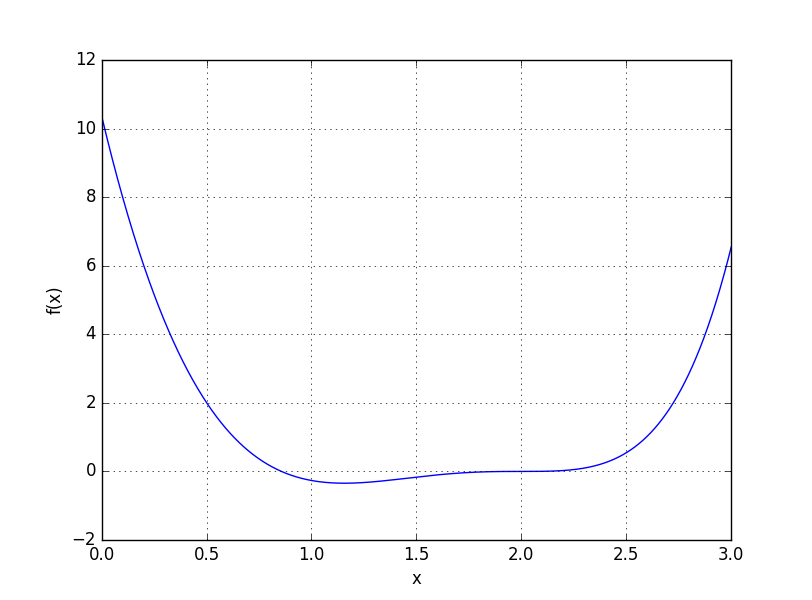
\includegraphics[width=\linewidth, height=9cm]{plot.png}
\end{center}

Καθώς η άσκηση δεν το απαιτεί δεν υπάρχουν έλεγχοι για σφάλματα
ούτε συνθήκες τερματισμού σε περίπτωση που δεν υπάρχουν ρίζες.

Ακολουθεί η συνάρτηση για διχοτόμηση:
\lstinputlisting[firstline=26, lastline=41]{ex1.py}

Απλά γίνετε η εγαρμογή του θεωρήματος για
$N = {{\ln{b-a} - \ln{error}}\over{\ln{2}}}$ φορές

Στην συνέχεια έχω τη συνάρτηση για την μέθοδο Newton-Raphson:
\lstinputlisting[firstline=42, lastline=55]{ex1.py}

Εδώ αρχικοποιώ τον πίνακα \texttt{temp\_l} με την τιμή
εισόδου της συνάρτησης και το αποτέλεσμα μιας πρώτης εφαρμογής της
αναδρομικής συνάρτησης $$f(x_{n}) = f(x_{n-1}) - {{f(x_{n-1})} \over {f'(x_{n-1})}}$$
Στην συνέχεια με τον έλεγχο στο while η συνάρτηση θα τρέχει μέχρι να
επιτευχθεί η επιθυμιτή ακρίβεια (6 δεκαδικά ψηδία)

Επιστρέφω την ρίζα, τον αριθμό επαναλήψεων και το σημείο εκκίνησης.
\textcolor{mygray}{
\begin{footnotesize}
  Ο αριθμός επαναλήψεων είναι Ν-1 γιατί η αύξηση του δείκτη γίνεται
  στο τέλος του \texttt{while} ενώ ξεκινάει με τον δείκτη στο 1 αντι του 0
  για να μπορεί να γίνει ο έλεγχος
\end{footnotesize}}
\newpage
Ακολουθέι η συνάρτηση της μεθόδου της τέμνουσας:
\lstinputlisting[firstline=56, lastline=70]{ex1.py}

Η συνάρτηση είναι αντίστοιχη με αυτή της Newton-Raphson.
Χρειάζεται δύο αρχικές τιμές, και για να γίνει ο έλεγχος του \texttt{while},
υπολογίζω και την τρίτη σύμφωνα με την αναδρομική συνάρτηση
$$x_{n+1} = x_n - {{f(x_n)(x_n - x_{n-1})} \over {f(x_n) - f(x_{n-1})}}$$
Ο έλεγχος είναι ο ίδιος με την Newton-Raphson για να πετύχω τα
6 δεκαδικά ψηφία

Επιστρέφω την ρίζα, τον αριθμό επαναλήψεων καθως και τις 2 αρχικές τιμές.

\newpage
Ακολουθεί η έξοδος του προγράμματος όταν το τρέχω με τις
κατάλληλες αρχικές τιμές (βασισμένες στο διάγραμμα την συνάρτησης):

\begin{lstlisting}[language=C, mathescape=true]
$\dollar$ python ex1.py
++++ Bisection ++++

Root in [0.00,1.50] after 22 loops: f(0.857143) = -0.000000

Root in [1.50,3.00] after 22 loops: f(2.000004) = 0.000000

++++ Newton - Raphson ++++

Starting at 1.00:
after 5 iterations the root is: f(0.857143) = -0.000000

Starting at 3.00:
after 29 iterations the root is: f(2.000011) = 0.000000

++++ Interpolation ++++

Root found in [0.70,0.90] after 11 iterations:
f(0.857143) = -0.000000

Root found in [1.70,2.10] after 52 iterations:
f(2.000023) = 0.000000
\end{lstlisting}

\newpage
Στο διάγραμμα που ακολουθεί βλέπουμε τις επαναλήψεις που
χρειάζετε η μέθοδος Newton-Raphson σε σχέση με την αρχική τιμή
που δίνεται

\begin{center}
  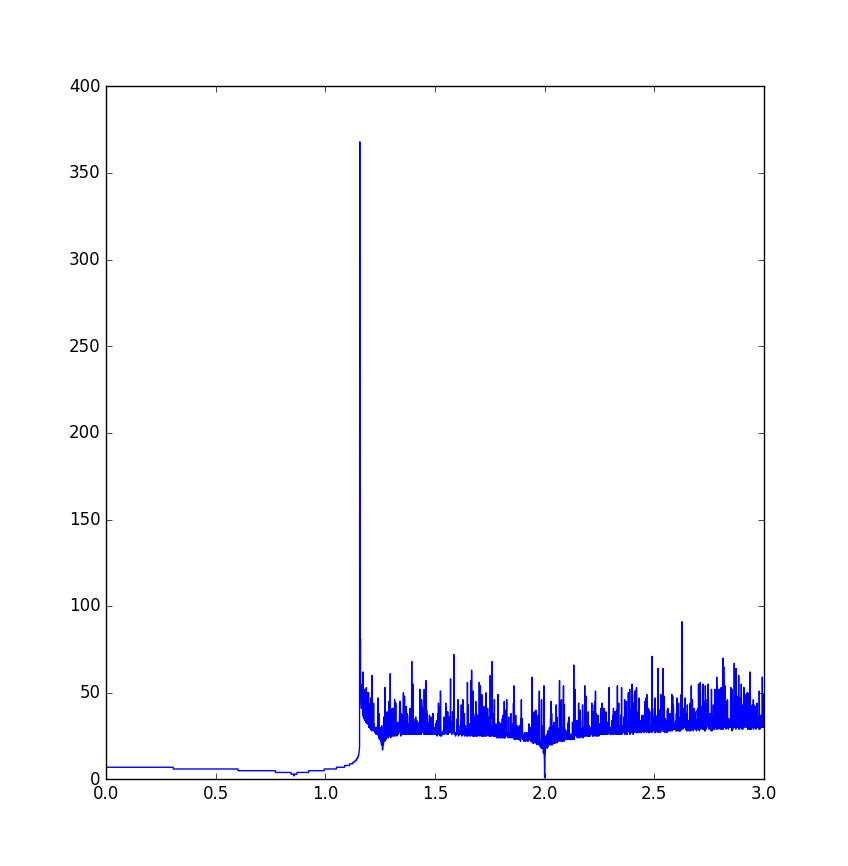
\includegraphics[scale = 0.7]{starting_point-loops.png}
\end{center}

Παρατηρώ οτι για την ρίζα στο $0.857143$ η μέθοδος συγκλίνει τετραγωνικά
ενώ για την ρίζα στο $2.000004$ θέλει εμφανώς περισσότερες επαναλήψεις.

Συγκρίνοντας αυτό το διάγραμμα με το plot της συνάρτησης στην 1η σελίδα
παρατηρώ οτι η ταχύτητα σύγκλισης στην πρώτη ρίζα είναι μεγάλη γιατι η
συνάρτηση διατηρεί την ίδια κυρτώτητα ενώ στην δεύτερη η συνάρτηση αλλάζει.

Καθώς η μέθοδος N-R χρησιμοποιεί την κλίση της παραγόγου για να βρεί το
επόμενο $x$ στην αναδρομή, όταν η κυρτώτητα αλλάζει γύρω απο την ρίζα
ο αλγόριθμος ταλαντώνετε και αργεί να συγκλίνει σε έναν αριθμό που να ικανοποιεί
το σφάλμα που θέσαμε.


\end{document}

%%% Local Variables:
%%% coding: utf-8
%%% mode: latex
%%% TeX-engine: xetex
%%% End:
\section{Άσκηση 2}


Ο κώδικας σε αυτήν την άσκηση είναι παρόμοιος με τον κώδικα της πρώτης
με το μόνο άξιο σχολιασμού να είναι η τροποποιημένη μέθοδος της τέμνουσας:
\lstinputlisting[firstline=58, lastline=74]{ex2/ex2.py}

καθως η άσκηση λέει πως το $x_{n+3}$ αντικαθιστά το $x_n$
δημιουργώ έναν πίνακα 3 θέσεων και χρησιμοποιώ τον τελεστή $\%$
για να γίνεται αυτη η αντικατάσταση κυκλικά

\subsection{Ερώτημα 1}

Ακολουθούν τα αποτελέσματα με κατάλληλες αρχικοποιήσεις:
\begin{lstlisting}[language=C, mathescape=true]
$\dollar$ python ex2/ex2.py
++++ almost-Bisection ++++

Root in [0.80,0.90] after 25 loops: f(0.841067) = 0.000000

Root in [0.95,1.10] after 7 loops: f(1.047667) = 0.000000

Root in [2.30,2.80] after 25 loops: f(2.300524) = 0.000000

++++ almost-Newton - Raphson ++++

Starting at 0.80:
after 4 iterations the root is: f(0.841069) = 0.000000

Starting at 1.00:
after 6 iterations the root is: f(1.044162) = -0.000000

Starting at 2.50:
after 4 iterations the root is: f(2.300524) = -0.000000

++++ almost-Interpolation ++++

Starting points: [1.00, 2.00, 3.00]. After 10 iterations:
f(1.043381) = -0.000000

Starting points: [0.70, 0.80, 0.90]. After 10 iterations:
f(0.841069) = -0.000000

Starting points: [2.20, 2.30, 2.40]. After 4 iterations:
f(2.300524) = 0.000000
\end{lstlisting}

%%% Local Variables:
%%% mode: latex
%%% TeX-master: "../master"
%%% End:

\section{Άσκηση 3}
\subsection{Ερώτημα 1}
Έχω υλοποιήσει σε \texttt{python} ένα πρόγραμμα που διαβάζει 2 αρχεία:
το \texttt{a.csv} με έναν $n\times n$ πίνακα $\mathbf{A}$ και το \texttt{b.csv} με έναν
$1\times n$ πίνακα $\mathbf{b}$ και κάνει την $\mathbf{LU}$ ανάλυση του $\mathbf{A}$
και στην συνέχεια βρίσκει την λύση στο σύστημα $\mathbf{Ax} = \mathbf{b}$

Διαβάζει τα αρχεία και φτιάχνει τους πίνακες $\mathbf{A}$ και $\mathbf{b}$
και ταυτόχρονα αρχικοποιεί τον πίνακα $\mathbf{L}$ σαν έναν $I_n$ και $\mathbf{U}$
όπου είναι ίδιος με τον $\mathbf{A}$ καθως είναι αυτός πάνω στον οποίο θα γίνουν
οι προσθαφαιρέσεις γραμμών αργότερα.

Στην συνέχεια βρίσκει τον τελικό πίνακα $\mathbf{U}$ και ταυτόχρονα συμπληρώνει
τον $\mathbf{L}$ με τους διαιρέτες. Μετά βρίσκει την λύση του συστήματος
$\mathbf{Ly} = \mathbf{b}$ και τέλος το $\mathbf{Ux} = \mathbf{y}$

Τυπώνει όλους τους πίνακες που χρειάστηκε καθώς και τον $\mathbf{A*x}$ για
επιβεβαίωση του σωστού αποτελέσματος.

Το αρχείο \texttt{a.csv} πρέπει να περιέχει $n$ νούμερα ανα σειρά χωρισμένα με
\texttt{space} και $n$ σειρές ενώ το \texttt{b.csv} $n$ σειρές απο 1 νούμερο.

%%% Local Variables:
%%% mode: latex
%%% TeX-master: "../master"
%%% End:

\subsection{Ερώτημα 2}

Σε αυτό το ερώτημα το πρόγραμμα διαβάζει τον πίνακα
απο ένα αρχείο \texttt{cho.csv}
και καλεί την μέθοδο \texttt{cholesky(A)} η οποία τυπώνει την ανάλυση
Cholesky αυτού του πίνακα. 


%%% Local Variables:
%%% mode: latex
%%% TeX-master: "../master"
%%% End:

\subsection{Ερώτημα 3}

Εδώ ο πίνακας $\mathbf{Α}$ και $\mathbf{b}$ δημιουργείτε απο το πρόγραμμα.

Η μεταβλητή \texttt{size} στην γραμμή 38 ελέγχει το $n$.
Στην συνέχεια καλείτε η συνάρτηση \texttt{GS(A, b)} η οποία επιστρέφει τον
πίνακα $x$.

%%% Local Variables:
%%% mode: latex
%%% TeX-master: "../master"
%%% End:

\end{document}

%%% Local Variables:
%%% mode: latex
%%% TeX-master: t
%%% End:
